\documentclass[letterpaper,11pt]{article}
\usepackage{fancybox}
\usepackage{graphicx}
\usepackage{tikz}
\usepackage{qtree}
\usepackage{fullpage}
\usepackage{amsmath}
\usepackage{amsthm}
\usepackage{amsfonts}
\usepackage{algorithm2e}
\usepackage{url}
\usepackage{cite}
\usepackage{fancyhdr}
\pagestyle{fancy}
\usepackage[utf8]{inputenc}
\usepackage[english]{babel}
\usepackage[nottoc]{tocbibind} %Adds "References" to the table of contents
%Document title, author and date (empty)
\title{Range Trees}
\author{Lumi Halitjaha}
\date{12/11/2017}
%Beginning of the document
\begin{document}

\maketitle

Range searching problems are problems that, typically, have the following form: \textit{Let $S$ be a set of points in $\mathbb{R}^d$, how do we pre-process the set $S$ so that we can quickly report and count the points inside a specific query region?}\cite{chazelle1999advances} Common data structures used to solve this type of problems are Sequential Scans, Projections, Cells, $k$-$d$ trees, $k$-ranges, and Range trees.\cite[p.~398]{Friedman} In this write-up I will discuss Range trees(usually referred to as \textit{Orthogonal Range Trees})

Range trees are balanced binary trees in which each node has an additional structure attached to it.\cite{sturzurange} They have been independently invented by D. E. Willard, J. L. Bentley, D. T. Lee and C. K. Wong, and G. S. Lueker.\cite{willard}\cite[p.~404]{Friedman} More formally, \textit{a range tree is a static structure that supports $d$-dimensional orthogonal range queries in a set of $d$-dimensional points.}\cite{brass2008advanced} Range trees are defined recursively. The recursion is on the dimensions of the tree, that is, the range tree of $n$ dimensions is defined in terms of the $(n-1)$-dimensional range tree.\cite[p.~404]{Friedman}
\begin{figure}[ht!]
\centering
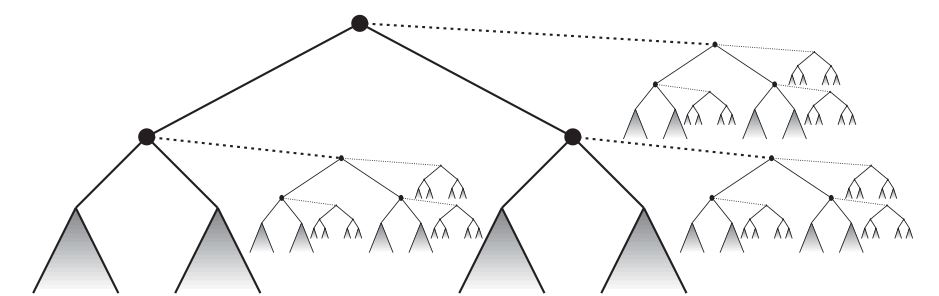
\includegraphics[width=90mm]{range_tree.JPG}
\caption{An example of a $3$-dimensional range tree: Each node has an associated  $2$-dimensional tree, in which each node has an associated $1$-dimensional tree.\cite[p.~183]{brass2008advanced} \label{overflow}}
\end{figure}

To build a Range tree with $d$ dimensions, we first build a $1$-dimensional tree by inserting each of the $n$ first coordinate points. We attach to each node a $(d-1)$-dimensional range tree data structure to store the other coordinates(dimensions) of the point, thus making the cost of building the tree $O(n(\log n)^d)$.\cite[p.~183]{brass2008advanced} As can be seen in figure 1, each tree is represented as a $1$-dimensional tree of $n$ nodes, with  $d-1$-dimensional trees attached to each of these nodes, so we need $O(n)$ time to build the one dimensional tree first, and then attach the $(d-1)$-dimensional trees to each node. Thus, the space complexity of a $d$-dimensional tree is $O(n(\log n)^{d-1})$.\cite[p.~183]{brass2008advanced}

Let us now consider the query time for range trees. In a $1$-dimensional binary tree, the cost of looking up a node is $O(\lg n)$.\cite[p.~292]{clrs}. To find the coordinates of a point in a range tree, however, we need to find all the different coordinates of the point. So it takes us $O(\lg n)$ time to find the first coordinate, then we search for the other dimensions(coordinates) of the point in the $(d-1)$-dimensional tree extending from each node, thus for each coordinate, we need to search a different one dimensional tree. Since the range searching problem requires us to output the points in an 
\newpage
\vspace*{0.2cm}
interval, it takes $O(1+k)$ time to list all the nodes belonging to the canonical interval decomposition. Therefore, the running time is $O((\log n)^d + k)$ if we are asked to output $k$ points.\cite[p.~183]{brass2008advanced} Can we query faster? Yes. Since the $1$-dimensional range tree is just a binary search tree, we can't do better than $\Omega (n \log n)$, because we are limited by the comparison-based model for one dimensional searching.\cite[p.~292]{clrs} \cite[p.~184]{brass2008advanced} But we can improve the query time of a $2$-dimensional range tree using the technique of fractional cascading which reduces the time complexity from $O(\log n)^2 + k)$ to $O(\log n + k)$.\cite[p.~184]{brass2008advanced}
One major advantage of range trees is that they achieve the best worst-case search time compared to the above-mentioned data structures used for range searching.\cite{Friedman} A disadvantage of this data-structure, though, is the high pre-processing and storage costs.\cite[p.~404]{Friedman} For small files that need to be searched few times, range trees are inferior to Sequential scan. In addition, $k$-$d$ trees perform better than range trees in practice since a range tree is practical mainly when it has up to $3$ dimensions.\cite[p.~405]{Friedman}

Nevertheless, Range trees have numerous applications. In many problems in computational geometry, range trees are used for reducing the time complexity of the solutions.\cite{sturzurange} Below are two problems that can be solved using range trees:\\
\textbf{1.} Given $N$ segments in a $2-D$ plane, parallel with the $x$ and $y$-axis, we want to determine the number of intersections between them. This problem can be solved using a sweep-line list(a collection of segments that intersect the sweep line) which is implemented via a range tree.\cite{sturzurange}\\
\textbf{2.} Assume a health-care company is introducing a health plan for all the users who are between $50$ and $70$ years old, and earn less than $100K$, and needs to have access to this category of users. We can solve this problem using a two-dimensional range tree whose dimensions are the users' incomes and their age. Using a $2-D$ range tree we can find in a very short time the users that fall into this range.\\

\bibliographystyle{abbrv}
\bibliography{references}
\end{document}
